\documentclass[journal]{IEEEtran}

\usepackage[T1]{fontenc}
\usepackage{cite}
\usepackage{amsmath,amssymb,amsfonts}
\usepackage{graphicx}
\usepackage{xcolor}
\usepackage{booktabs}
\usepackage{array}
\usepackage[hidelinks]{hyperref}

\newcommand{\mbf}[1]{\mathbf{#1}}
\newcommand{\bs}[1]{\boldsymbol{#1}}
\newcommand{\todo}[1]{\textcolor{red}{[#1]}}

\begin{document}

\title{Latency-Aware Phase Optimization for Reconfigurable Intelligent Surfaces Serving Mobile Users}

\author{Seda~Savaşçı~Şen, Ali~Çalhan, and Murtaza~Cicioğlu%
\thanks{(Corresponding author: Seda Savaşçı Şen.)}%
\thanks{S.~Savaşçı~Şen is with the Department of Electrical and Electronics Engineering, Düzce University, Düzce, Türkiye (e-mail: sedasavascisen@duzce.edu.tr).}%
\thanks{A.~Çalhan is with the Department of Computer Engineering, Düzce University, Düzce, Türkiye (e-mail: alicalhan@gmail.com).}%
\thanks{M.~Cicioğlu is with the Department of Computer Engineering, Bursa Uludağ University, Bursa, Türkiye (e-mail: murtazacicioglu@uludag.edu.tr).}}

\markboth{IEEE Transactions on Wireless Communications}%
{Latency-Aware Phase Optimization for RIS Serving Mobile Users}

\maketitle

\begin{abstract}
Phase optimizers for reconfigurable intelligent surfaces (RISs) are usually compared by their rate on the given channel, although a walking user changes the channel within tens of milliseconds. We evaluate each method by its \emph{effective rate}, the rate on the channel at the end of its computation, with measured latencies, in a narrowband indoor multi-user multiple-input single-output downlink with a 32-element RIS, perfect channel knowledge and a freshly computed precoder. First, coordinate descent and long-run Adam, despite high initial-channel rates, require 0.9--5.9~s and trail, at deployment, a single-user heuristic taking 2.5~ms. Second, the effective rate has an interior maximum in the number of iterations: at 1.5~m/s it lies at four to six Adam steps, and 48 steps lower it by 14\%. This optimum is governed by the step time relative to the Doppler frequency, falling from eight steps at 3~km/h to one at 30~km/h; a small-delay model shows that such an optimum exists for every nonzero step time and, with fitted constants, explains its scaling. Third, a learned update rule that outperforms tuned Adam at equal iteration counts is dominated by faster, better Adam configurations at latencies measured on one processor thread.
\end{abstract}

\begin{IEEEkeywords}
Reconfigurable intelligent surface, phase optimization, mobility, channel aging, computation latency.
\end{IEEEkeywords}

\section{Introduction}
\label{sec:intro}

\IEEEPARstart{A}{} reconfigurable intelligent surface (RIS) can extend coverage to blocked areas of a building~\cite{Basar2019Access,DiRenzo2020JSAC,Wu2021TCOM}; a 256-element RIS has served as a transmit antenna~\cite{Dai2020Access}, and another prototype has strengthened a link through a concrete wall~\cite{Pei2021TCOM}. Its benefit, however, depends on configuring the passive elements for the user's current channel rather than for a past one. Choosing those phases is a hard, non-convex problem, attacked with iterative solvers~\cite{Wu2019TWC,Abeywickrama2020TCOM,Pan2020TWC,Guo2020TWC,Choi2024TCOM} and, increasingly, with learned policies~\cite{Huang2020JSAC}. These methods are usually compared by the rate they reach on the channel they were given.

Such a comparison neglects the time the optimization itself requires. A pedestrian user changes the radio channel within tens of milliseconds, whereas an iterative solver may require seconds; when its solution becomes available, the channel for which it was computed has already changed. A coarse phase configuration delivered within the coherence time can therefore outperform a near-optimal one delivered later, and additional iterations can reduce, rather than increase, the achieved rate.

This paper quantifies this effect. We evaluate every method on the channel that exists when it finishes, its \emph{effective rate}, with latencies measured on a CPU, in an indoor office with walking users and the 3GPP TR~38.901 channel model~\cite{3gpp_channel}. We address the question a base station (BS) faces in this setting: once computation time is accounted for, which method should it run, and for how many iterations? It continues our single-pass phase predictor with a sine--cosine representation~\cite{SavasciSen2026AISY} by examining when such speed is beneficial once run time is charged.

\subsection{Contributions}
\begin{enumerate}
    \item We introduce the effective rate, which evaluates each optimizer on the channel at its measured completion time (Section~\ref{sec:framework}), and show that, for pedestrian users at the measured step cost, the solvers with the highest initial-channel rate are outperformed by a single-user heuristic that requires milliseconds.
    \item We show that the effective rate has an interior maximum in the number of iterations, governed by a single quantity, the step time relative to the Doppler frequency. A small-delay model (Proposition~1) shows that an interior optimum exists for every nonzero step time and, with fitted constants, explains how it scales, so the step count should be adapted to the user speed and the step time. In the narrowband model the optimum persists for a second classical optimizer, a larger surface and every standardized indoor speed.
    \item For continuous re-optimization at the BS, we show that the pilot overhead determines the update period and that updates of at most 8 steps suffice.
    \item We compare a learned update rule with a tuned classical optimizer both at equal steps and at equal measured latency, and show that its per-step advantage is reversed once each step is charged its measured time.
    \item We quantify the dependence of the results on the assumption that the BS refreshes its precoder from the current channel, and evaluate the effects of pilot airtime, estimation error and discrete phases.
\end{enumerate}

\section{Related Work}
\label{sec:related_work}

\emph{RIS phase optimization.} Joint precoding and phase design has been addressed with alternating optimization and semidefinite relaxation~\cite{Wu2019TWC}, practical phase-dependent amplitude models~\cite{Abeywickrama2020TCOM}, block coordinate descent~\cite{Pan2020TWC}, fractional programming~\cite{Guo2020TWC}, fixed-point and manifold methods~\cite{Yu2019ICCC} and weighted minimum mean-square error (WMMSE) methods~\cite{Choi2024TCOM} built on the algorithm of~\cite{Shi2011TSP}. These works report the objective value reached; run time is usually a complexity order, and where it is measured, on fixed channel realizations~\cite{Abeywickrama2020TCOM,Yu2019ICCC,Shi2011TSP,Cao2022TWC}, it is not compared with the coherence time.

\emph{Learning.} Learned policies include deep reinforcement learning for joint precoding and phase design~\cite{Huang2020JSAC} and learning to reflect directly from pilots~\cite{Jiang2021JSAC}. Algorithm unrolling turns an optimizer's iterations into network layers~\cite{Monga2021SPM}; it has been applied to RIS beamforming~\cite{Liu2022TWC}, MIMO detection~\cite{Samuel2019TSP} and WMMSE precoding~\cite{Hu2021TWC,Pellaco2022OJCOMS}, and trained networks can approximate WMMSE at a fraction of its run time~\cite{Sun2018TSP}. Predicting the sine and cosine of each phase removes the $\pm\pi$ discontinuity of direct phase regression~\cite{SavasciSen2026AISY}. Learned methods are usually motivated by speed, but that speed is rarely related to how fast the channel changes; even when both are timed on one machine~\cite{Samuel2019TSP,Sun2018TSP,Hu2021TWC,Liu2022TWC}, the classical baseline runs to convergence or a fixed iteration count, not to the same latency.

\emph{Mobility and outdated channels.} A vehicle-mounted refracting surface with two-stage estimation turns fast fading into slow fading~\cite{Huang2022TWC}. Channel aging~\cite{Papazafeiropoulos2023TVT} and outdated channel knowledge~\cite{Zhang2022TCOM} have been analyzed for RIS, predictive beamforming points beams at the forecast positions of fast drones~\cite{Liu2021WCL}, and active sensing tracks mobile users~\cite{Han2025TWC}. Aging is classical in massive MIMO~\cite{Truong2013JCN,Chopra2018TWC}, as is limited channel feedback in broadcast channels~\cite{Jindal2006IT}. Two-timescale designs update the phases from channel statistics and the precoder from instantaneous channels~\cite{Zhao2021TWC,Cao2022TWC}. Practical surfaces have a few bits of phase resolution~\cite{Wu2020TCOM,Zhao2024OJCOMS}; Section~\ref{sec:res_robust} adds 1--3-bit phases to our continuous-phase results. In these works the delay between channel acquisition and use, where modeled, is fixed, even where computation is named as a cause~\cite{Truong2013JCN}; the optimizer's own run time is at most a feasibility check or a fixed overhead~\cite{Ryu2026arXiv,Liu2021WCL} and does not enter the aging.

\begin{table*}[t]
\caption{Treatment of channel variation and optimizer run time in representative works.}
\label{tab:literature}
\footnotesize
\setlength{\tabcolsep}{4pt}
\begin{tabular}{@{}>{\raggedright\arraybackslash}p{0.13\textwidth}>{\raggedright\arraybackslash}p{0.22\textwidth}>{\raggedright\arraybackslash}p{0.22\textwidth}>{\raggedright\arraybackslash}p{0.17\textwidth}>{\raggedright\arraybackslash}p{0.19\textwidth}@{}}
\toprule
Work & Problem & Channel variation & Run time & Role of run time \\
\midrule
\cite{Pan2020TWC,Guo2020TWC,Choi2024TCOM} & RIS precoding and phases (block coordinate descent, fractional programming, WMMSE) & none & complexity order & none \\
\cite{Abeywickrama2020TCOM,Yu2019ICCC} & RIS beamforming (practical phase model; fixed-point and manifold methods) & none & measured on a fixed channel & not compared with the coherence time \\
\cite{Sun2018TSP,Liu2022TWC} & neural network imitating WMMSE; unfolded RIS design & none; CSI delay swept over 0--1.2~ms~\cite{Liu2022TWC} & measured for learned and classical methods & not related to channel variation; classical method at convergence or fixed iterations \\
\cite{Cao2022TWC} & RIS, two-timescale design & first-order aging, fixed delay & measured per iteration & not part of the delay \\
\cite{Papazafeiropoulos2023TVT,Zhang2022TCOM} & RIS with aged or outdated channels & Jakes correlation; delay set by the frame or estimation & complexity order or closed form & none \\
\cite{Truong2013JCN} & massive MIMO channel aging & fixed delay (1--10~ms); computation named as a cause & not measured & none \\
\cite{Han2025TWC} & RIS beam tracking, learned active sensing & Gauss--Markov, fixed block & complexity order & none \\
\cite{Liu2021WCL} & predictive beamforming for drones & prediction one 20~ms slot ahead & measured (2~ms) & feasibility check \\
\cite{Ryu2026arXiv} & RIS, sensing-aided optimization & fixed delay & estimated from operation counts & constraint and fixed overhead \\
This work & RIS, multi-user MISO & walking users; channel at measured completion time & measured (one thread) & enters the aging; methods compared at equal latency \\
\bottomrule
\end{tabular}
\end{table*}

\emph{Gap.} Table~\ref{tab:literature} summarizes how representative works treat channel variation and run time. To our knowledge, no RIS work evaluates each method on the channel at its own measured completion time, shows that this creates an optimal iteration count, or compares learned and classical optimizers both at equal steps and at equal measured time.

\section{System and Channel Model}
\label{sec:system}

\subsection{Signal Model}
A BS with a uniform linear array of $N_t=8$ half-wavelength-spaced antennas serves $K=4$ single-antenna users through a direct link and an RIS of $N=32$ passive elements (an $8\times 4$ planar array); Section~\ref{sec:res_scaling} also uses $N=64$. With phases $\bs{\theta}\in[0,2\pi)^N$, $\mbf{v}=e^{j\bs{\theta}}$ and precoder $\mbf{W}=[\mbf{w}_1,\dots,\mbf{w}_K]$, user $k$ receives
\begin{equation}
    y_k = \left(\mbf{h}_{d,k}^H + \mbf{g}_k^H \operatorname{diag}(\mbf{v})\mbf{F}\right)\sum_{j=1}^K \mbf{w}_j s_j + n_k ,
    \label{eq:signal}
\end{equation}
where $\mbf{F}\in\mathbb{C}^{N\times N_t}$ is the BS--RIS channel, $\mbf{g}_k^H$ the RIS--user channel, $\mbf{h}_{d,k}^H$ the direct channel and $n_k\sim\mathcal{CN}(0,\sigma^2)$. With $\mbf{h}_k^H(\bs{\theta})$ the bracketed effective channel, user $k$ has rate $R_k=\log_2(1+\mathrm{SINR}_k)$, with signal-to-interference-plus-noise ratio $\mathrm{SINR}_k = |\mbf{h}_k^H \mbf{w}_k|^2/(\sum_{j\ne k}|\mbf{h}_k^H \mbf{w}_j|^2 + \sigma^2)$. The precoder is regularized zero-forcing~\cite{Peel2005TCOM} on the effective channel, with regularizer $\lambda = K\sigma^2/P$ and total power $P$. The objective is the minimum user rate, a fairness criterion also used for RIS-assisted multiple-input single-output (MISO) systems in~\cite{Nadeem2020TWC},
\begin{equation}
    \max_{\bs{\theta}} \; \min_k R_k(\bs{\theta}),
    \label{eq:maxmin}
\end{equation}
which Adam, Armijo and the learned update (Section~\ref{sec:method}) optimize through the smooth surrogate $-\tfrac{1}{\beta}\log\sum_k e^{-\beta R_k}$, $\beta=8$; coordinate descent and the long-run Adam reference maximize the hard minimum.

\subsection{Geometry and Propagation}
\begin{figure*}[t]
\centering
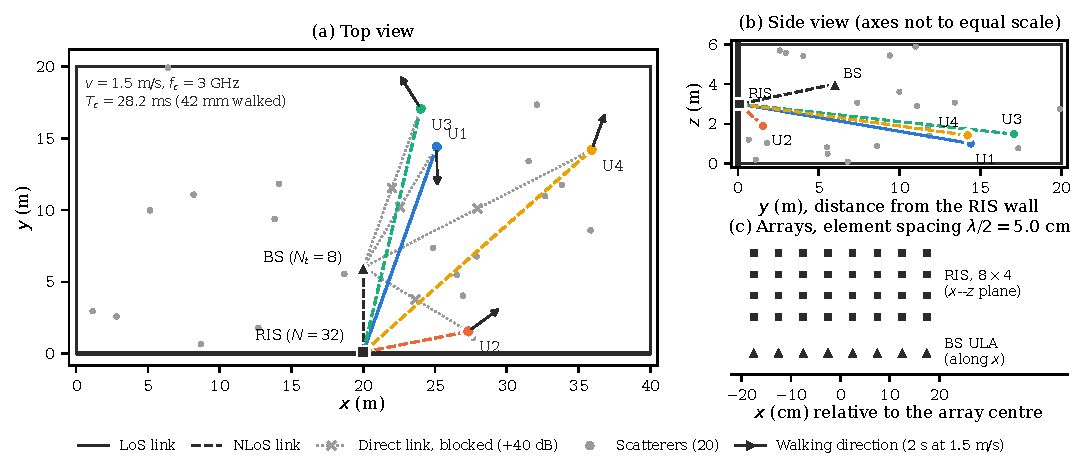
\includegraphics[width=\textwidth]{figures/fig_scenario.pdf}
\caption{The simulated scenario (first scenario of the aging set). (a)~Top view of the $40\times20\times6$~m office: BS at $(20,6,4)$~m, wall-mounted RIS centered at $(20,0.1,3)$~m, four users walking at 1.5~m/s, 20 point scatterers. Line style: line-of-sight (LoS) state of each link. All direct links carry the 40~dB blockage. Arrows: 2~s of walking; within one coherence time a user moves only 42~mm. (b)~Side view. (c)~Element layouts.}
\label{fig:scenario}
\end{figure*}
The room is $40\times 20\times 6$~m (Fig.~\ref{fig:scenario}). The RIS is centered at $(20, 0.1, 3)$~m on a wall; the BS is at $(20, 6, 4)$~m, in the panel's boresight and beyond its Fraunhofer distance. Users are dropped uniformly at heights of 1--2~m. The carrier is $f_c=3$~GHz, the bandwidth 20~MHz, the transmit power 20~dBm, the BS antenna gain 5~dBi and the noise figure 7~dB. All links follow the 3GPP TR~38.901 indoor-office model~\cite{3gpp_channel}: its path loss, mixed-office LoS probability, Rician factor and log-normal shadowing with exponential spatial correlation at 5~m (TR~38.901 specifies 10~m for LoS and 6~m for non-LoS). Non-LoS components come from point scatterers shared by all links of a scenario. The cascaded amplitude follows the free-space two-hop model of~\cite{Tang2021TWC} with a $\cos^q$ power pattern ($q{=}1$); we add the TR~38.901 excess loss and shadowing to each hop. Our element gain, $2(2q{+}1)$, exceeds Tang's $2(q{+}1)$; the latter lowers absolute rates by about 5\% and leaves $L^\star$ and the best method unchanged. Because an RIS is deployed where the direct path is obstructed, the direct link carries an extra 40~dB of loss.

\subsection{Mobility}
Users walk in straight lines at $v=1.5$~m/s (5.4~km/h) and are reflected off the walls. This lies between the 3~km/h of the 3GPP indoor-hotspot evaluation~\cite{3gpp_tr38913} and the 10~km/h upper end of the IMT-2020 pedestrian class, at which indoor mobility is evaluated~\cite{itu_m2410}; Section~\ref{sec:res_sensitivity} repeats the main measurements at these and higher speeds. Scatterers, path gains, LoS states, shadowing and $\mbf{F}$ are held fixed; only the users move, and $\mbf{g}_k(t)$ and $\mbf{h}_{d,k}(t)$ are recomputed from geometry at every instant. The reference time scale is the Doppler frequency $f_d=vf_c/c=15$~Hz, with coherence time $T_c=\sqrt{9/(16\pi)}/f_d\approx0.423/f_d=28.2$~ms.

\emph{Limitations.} Fixed scatterers make the channel change less than a real one over seconds, so effective rates beyond 200~ms are optimistic for slow methods; the true values should lie between them and the stale floor of Table~\ref{tab:aging}. Scattered-path gains are drawn independently per BS antenna, which makes all absolute rates optimistic; Section~\ref{sec:res_sensitivity} repeats the main measurements with shared gains. In the main results, channel knowledge is perfect apart from the acquisition delay we add; Section~\ref{sec:res_robust} adds estimation error. The model is narrowband (no beam squint), and far-field for $N=32$; for $N=64$ the BS (6.0~m away) lies just inside the 6.4~m Fraunhofer distance, and the channel uses exact per-element distances.

\section{Latency-Aware Evaluation Framework}
\label{sec:framework}

\subsection{Effective Rate}
Let a method $A$ receive the channel $\mathcal{H}(0)=\{\mbf{F},\mbf{g}_k(0),\mbf{h}_{d,k}(0)\}$, return the phase $\bs{\theta}_A$, and need the wall-clock time $\tau_A$ to do so.

\textbf{Definition 1 (Effective rate).} The effective rate of $A$ is its minimum user rate on the channel that exists when it finishes,
\begin{equation}
    R^{\mathrm{eff}}_A = \min_k R_k\big(\bs{\theta}_A;\,\mathcal{H}(\tau_A)\big),
    \label{eq:effective_rate}
\end{equation}
with the precoder recomputed from $\mathcal{H}(\tau_A)$.

The precoder is a closed-form computation that the BS repeats whenever it has fresh pilots; the RIS phase needs the iterative optimization whose latency we measure. Definition~1 therefore lets the phase age and keeps the beam fresh, a split similar to that of two-timescale designs~\cite{Zhao2021TWC}. Sections~\ref{sec:res_beam} and~\ref{sec:res_robust} price this assumption.

\subsection{Why an Optimal Number of Steps Exists}
For an iterative method run for $L$ steps, write $r_0(L)$ for its minimum rate at $t=0$, $\tau(L)$ for its latency, and $\Delta(L)=r_0(L)-\min_k R_k(\bs{\theta}_L;\mathcal{H}(\tau(L)))$ for the rate lost to aging during its own run time, so that $R^{\mathrm{eff}}(L)=r_0(L)-\Delta(L)$. Each step raises $r_0$ with diminishing returns, while $\Delta$ grows with $\tau$. A step pays off only while
\begin{equation}
    r_0(L+1)-r_0(L) \;>\; \Delta(L+1)-\Delta(L),
    \label{eq:marginal}
\end{equation}
and the effective rate peaks where this fails: the \emph{intrinsic optimum} $L^\star$. It depends jointly on the optimizer, its per-step latency and the rate of channel variation. Whether $R^{\mathrm{eff}}$ is unimodal is an empirical question (Section~\ref{sec:res_optimum}).

\subsection{Equal Steps versus Equal Milliseconds}
If one learned step costs as much time as $c$ classical steps, an equal-step comparison gives the learned method $c$ times the time budget. We therefore also compare at equal measured time.

\textbf{Definition 2 (Dominance).} Configuration $B$ dominates $A$ if $\tau_B\le\tau_A$ and $r_{0,B}\ge r_{0,A}$, with one inequality strict.

A dominated configuration is never the better choice at any latency budget.

\subsection{Normalized Step Cost and a Small-Delay Model}
Channel variation depends on the distance a user moves in wavelengths, $f_d\tau$. If an optimizer takes $\Delta T$ per step, its latency after $L$ steps in these units is $Lx$, with
\begin{equation}
    x = \Delta T\, f_d .
    \label{eq:x}
\end{equation}
In our model, scaling $\Delta T$ is exactly equivalent to scaling the speed $v$; a change of carrier is only approximately equivalent, since the path loss and the array size in wavelengths change with it.

Two approximate regularities, checked in Section~\ref{sec:res_scaling}, make~\eqref{eq:marginal} explicit. The convergence gap decays roughly as a power law,
\begin{equation}
    R_\infty - r_0(L) \approx D\,L^{-\gamma},
    \label{eq:conv_law}
\end{equation}
and for small delays the aging loss is quadratic in the distance moved, $u=f_d\tau$,
\begin{equation}
    \Delta(L,u) \approx \kappa_L\, u^2 ,
    \label{eq:aging_law}
\end{equation}
as in the leading term of the Clarke correlation, $J_0(2\pi u)\approx 1-\pi^2u^2$~\cite{Clarke1968BSTJ}. With $u = xL$,
\begin{equation}
    R^{\mathrm{eff}}(L) \approx R_\infty - D\,L^{-\gamma} - \kappa\, x^2 L^2 .
    \label{eq:reff_model}
\end{equation}

\textbf{Proposition 1 (Scaling of the optimum).} For $\gamma, D, \kappa, x > 0$ and $\kappa_L=\kappa$, \eqref{eq:reff_model} has a unique maximizer over $L>0$,
\begin{equation}
    L^\star = \left(\frac{\gamma D}{2\kappa}\right)^{\frac{1}{\gamma+2}} x^{-\frac{2}{\gamma+2}} ,
    \label{eq:Lstar}
\end{equation}
at which the aging loss equals $\gamma/2$ times the remaining convergence gap.

\emph{Proof.} The derivative $\gamma D L^{-\gamma-1} - 2\kappa x^2 L$ is positive for small $L$, negative for large $L$, and vanishes only at $L^{\gamma+2}=\gamma D/(2\kappa x^2)$; the second derivative is negative. Substituting gives the balance. \hfill$\square$

The optimum is thus a power law in $x$ with exponent in $(-1,0)$: a faster optimizer should run more steps, but less than proportionally more. The derivation assumes $xL^\star \ll 1$, which holds over our range ($xL^\star\le 0.16$). With fitted constants, \eqref{eq:Lstar} describes the measurements rather than predicting them independently; its value lies in explaining how the optimum shifts.

\subsection{Periodic Re-optimization}
A deployed controller repeats the optimization with period $U$: it spends $T_{\mathrm{p}}$ on pilots, without data, then $L\Delta T$ on optimization, deploys the result and waits ($U \ge T_{\mathrm{p}}+L\Delta T$; \emph{back-to-back} means equality).

\textbf{Definition 3 (Time-averaged effective rate).} With $\bs{\theta}(t)$ the deployed phase and $\mathcal{P}$ the pilot intervals, over a window $\mathcal{W}$
\begin{equation}
    \bar{R}^{\mathrm{eff}} = \frac{1}{|\mathcal{W}|}\int_{\mathcal{W}\setminus\mathcal{P}} \min_k R_k\big(\bs{\theta}(t);\,\mathcal{H}(t)\big)\,dt .
    \label{eq:time_avg}
\end{equation}
Each update starts from scratch (\emph{cold}) or from the deployed phase (\emph{warm}).

\section{Measurement Protocol}
\label{sec:method}

\subsection{Scenario Sets}
All sets use seed 11 unless stated otherwise, and numbers from different sets are never mixed in one comparison.
\begin{itemize}
    \item \emph{Aging set} (Tables~\ref{tab:aging}--\ref{tab:tracking}, Figs.~\ref{fig:aging}--\ref{fig:scaling}): 400 scenarios with walking users and 20 point scatterers, close to the 15--19 clusters of the 3GPP indoor-office model; with $N=64$, the same construction with an $8\times 8$ panel.
    \item \emph{Beam set} (Section~\ref{sec:res_beam}): 400 more scenarios, 6 scatterers.
    \item \emph{Static set} (Fig.~\ref{fig:eqms}): 6000 static scenarios, randomly split 4200/900/900 (training/validation/test); the learned update is validated on 500, Adam on 400 of these (on all 500 it picks the same setting); results use 600 test scenarios.
\end{itemize}
The generator is not prefix-stable; trained models are evaluated at their training sample count.

\subsection{Methods}
\begin{table}[t]
\caption{Methods, settings and computation cost (aging set unless stated).}
\label{tab:hyper}
\footnotesize
\setlength{\tabcolsep}{3pt}
\begin{tabular}{@{}>{\raggedright\arraybackslash}p{0.2\columnwidth}>{\raggedright\arraybackslash}p{0.51\columnwidth}>{\raggedright\arraybackslash}p{0.23\columnwidth}@{}}
\toprule
Method & Settings & Cost \\
\midrule
SU-average & phase of the sum of the $K$ single-user alignments & 0.42~ms \\
SU-best-of & best of the $K$ alignments and SU-average & 2.5~ms \\
Adam & start SU-average; soft-min, $\beta=8$; step size 0.5 (static set: 0.75, selected for $L\le 16$); $L^\star=4$--6 at 1.5~m/s & 1.66~ms/step$^{a}$ \\
Armijo & start SU-average; soft-min; initial step 3, backtracking; $L^\star=4$ & 2.09~ms/step \\
Coordinate descent & 16 phase levels, hard min, 1--8 sweeps (best: 2) & 107~ms/sweep \\
Long-run Adam & Adam, step size 0.05, 1000 iterations, 3 random starts, hard min & 5.85~s \\
Learned update (static set) & $L\in\{1,2,4,8,16\}$, one network per $L$; 41 input channels; 272{,}835--272{,}850 parameters; unsupervised soft-min training (Adam, $10^{-3}$, cosine schedule, batch 32, 12 epochs) & 2.7--4.0 Adam steps per step \\
\bottomrule
\end{tabular}

\vspace{2pt}\raggedright\footnotesize $^{a}$1.66~ms in Sections~\ref{sec:res_aging}--\ref{sec:res_tracking}; 1.60--1.71~ms (static set) in Section~\ref{sec:res_reversal}; 1.33~ms (re-measurement) in Section~\ref{sec:res_robust}; other sessions: supplementary material.
\end{table}
\emph{SU-average} and \emph{SU-best-of} are closed-form single-user phase alignments; the latter keeps the best of $K{+}1$ candidates. \emph{Adam}~\cite{Kingma2015ICLR} optimizes the soft-min surrogate, starting from SU-average. \emph{Armijo} is steepest ascent with Armijo's rule~\cite{Armijo1966PJM} on the same surrogate, with a per-scenario backtracking line search. \emph{Coordinate descent} searches each element over 16 phase levels, for up to 8 sweeps; \emph{long-run Adam} runs 1000 iterations from 3 random starts. The \emph{learned update} is a deep-unfolded network with $L$ learned steps; one network is trained per $L$, without labels. For each user and element it receives 37 static input channels: the real and imaginary parts of the normalized RIS--user channel (2), of the BS--RIS channel at each of the $N_t$ antennas (16) and of the direct channel (16), the cosine and sine of the user's single-user alignment phase, and the logarithm of the user's relative channel power. At every step four dynamic channels are added: the cosine and sine of the current phase, the user's standardized rate and the normalized gradient of the soft-min rate. A convolutional and long short-term memory (LSTM) backbone along the elements, two layers that exchange information across users and a per-element head produce a phase update, scaled by a learned step size; the weights are shared across steps. Table~\ref{tab:hyper} lists the settings of all methods.

\emph{Tuning.} On the static set, Adam's step size and objective (soft-min or hard min) are selected on the validation set at every budget: from ten values in $[0.02, 2.0]$ for $L\le 16$, where 0.75 with the soft-min, an interior point, is selected every time, and from six values in $[0.2, 1.5]$ for $L=24$--$64$. On the aging set Adam uses step size 0.5 (0.25, 0.75 and 1.0 give lower peaks), and Armijo's initial step is chosen from five values (3 is selected); both choices use the reported scenarios, so they are robustness checks rather than held-out selections.

\subsection{Timing}
Latencies are wall-clock times for one scenario on an Intel Xeon CPU at 2.1~GHz with one PyTorch thread (except the two-thread 1.66~ms below), in unoptimized Python (Section~\ref{sec:res_scaling} considers a faster Adam step); the median over repetitions is kept, and most measurements are repeated in several rounds. Adam's step time appears with three values, each tied to one measurement session (Table~\ref{tab:hyper}). The aging-set results of Sections~\ref{sec:res_aging}--\ref{sec:res_tracking} use 1.66~ms (13.3~ms for 8 steps), from an earlier two-thread measurement made before a precoder fix; it lies within the 1.49--2.02~ms of later rounds on the aging set. The static-set comparison (Section~\ref{sec:res_reversal}) uses its own five-round medians, 1.60--1.71~ms per step. Section~\ref{sec:res_robust} uses a one-thread re-measurement of 1.33~ms (load average 0.45 before timing; coordinate descent 0.70~s); with it $L^\star=6$, $L=48$ costs 14.9\%, and SU-best-of stays ahead of 8-sweep coordinate descent by 0.26~b/s/Hz (CI 0.15--0.37; optimistic for coordinate descent), so the optimum and the cost of $L=48$ do not depend on which of the two aging-set values is used. Armijo costs 1.26 times as much as Adam per step (2.09~ms; per-scenario ratio 0.81--1.97). On the static set the learned network's input features are excluded from its time, which favors it. Other checks use separate sessions; load averages, round counts and spreads are in the supplementary material.

\subsection{Statistics and Pilots}
Effective rates are interpolated on a time grid at each method's latency plus an optional acquisition delay $T_{\mathrm{ov}}$. Evaluating at the exact latency instead changes Table~\ref{tab:aging} by at most 0.006~b/s/Hz within the reliable horizon (0.008 and 0.037 beyond it) and the Adam sweep of Fig.~\ref{fig:optimum} by at most 0.027; the optimum stays at 4--6 steps and the cost of $L=48$ becomes 14.2\%. Because absolute rates vary strongly across scenarios ($\pm$0.17--0.24~b/s/Hz for the means of Table~\ref{tab:aging}), methods are compared with paired bootstrap confidence intervals (CIs) over scenarios (2000 resamples). Differences of a few thousandths of a b/s/Hz between neighboring $L$ are not resolved. Best configurations are selected and reported on the same scenarios unless stated, without a multiple-comparison correction, and should be read as estimates.

We tie $T_{\mathrm{ov}}$ and the pilot time $T_{\mathrm{p}}$ to cascaded channel estimation~\cite{Zheng2022COMST}. With the uplink scheme of~\cite{Wang2020TWC} and TDD reciprocity, 48 pilot symbols suffice for $K=4$, $N=32$ and $N_t=8$ in the noise-free case. With 5G New Radio (NR) numerology~\cite{3gpp_nr_phy} and one orthogonal frequency-division multiplexing (OFDM) symbol per pilot they last 3.43, 1.71 and 0.86~ms at 15, 30 and 60~kHz subcarrier spacing; feedback, estimation processing and RIS switching come on top and are not modeled. The periodic controller is simulated on a 0.5~ms grid over 200~ms, with update periods of 10--80~ms or back-to-back, averaging over 100--200~ms; pilot airtime is charged as the fraction of each grid step it occupies, each phase takes effect at its exact deployment instant, and channel snapshots are taken at the nearest grid point.

\emph{Reproducibility.} One script generates every table and figure from stored result files, except Table~\ref{tab:tracking} (a corrected copy of the tracking simulation) and Section~\ref{sec:res_robust} (separate scripts); rerunning the aging sweeps reproduces them bit for bit. A separate audit script checks 126 assertions about the learning experiments of the underlying thesis; among the results here it covers those of Section~\ref{sec:res_sensitivity}.

\section{Results}
\label{sec:results}

\subsection{Effective Rates of Fast and Slow Solvers}
\label{sec:res_aging}
In this scenario the RIS carries most of the signal: with the direct links blocked, the median per-user signal-to-noise ratio (SNR) is 20.0~dB for the direct link alone and 31.1~dB through the RIS. Without the RIS the minimum user rate is 1.744~b/s/Hz; a random phase gives 4.072.

Fig.~\ref{fig:aging} fixes each method's phase at $t=0$ and follows the minimum rate as users walk. Rates hold for a few milliseconds, drop sharply around $T_c$ and level off above the stale floor. The more thoroughly a phase is optimized, the larger its loss: by $T_c$ long-run Adam falls from 7.117 to 5.473~b/s/Hz, while SU-average only moves from 4.624 to 4.503.

Table~\ref{tab:aging} evaluates each method at its own latency. Long-run Adam and coordinate descent have the best $t=0$ rates of the table, but they need 5.9~s and 0.88~s, respectively. By then users have moved up to several meters, and even their optimistic effective rates fall below that of SU-best-of, which takes 2.5~ms: SU-best-of is ahead of coordinate descent by 0.297~b/s/Hz (95\% CI 0.204--0.390) and of long-run Adam by 0.604 (0.415--0.805). This is not an artifact of a fixed budget: one multi-user coordinate sweep already takes 107~ms, about four coherence times, and the best of one to eight sweeps (5.014~b/s/Hz, two sweeps) stays 0.26~b/s/Hz below SU-best-of (CI 0.17--0.36).

\begin{table}[t]
\centering
\caption{Rate at $t=0$, latency and effective rate (aging set, 400 scenarios, 1.5~m/s). Stale floor: $t=0$ phase on an independent channel. $^\dagger$Beyond the 200~ms reliable horizon; optimistic. $^\ast$Value at the last grid point (5.6~s).}
\label{tab:aging}
\footnotesize
\begin{tabular}{lrrrr}
\toprule
Method & $t{=}0$ & Latency & Effective & Stale \\
 & (b/s/Hz) & (ms) & (b/s/Hz) & (b/s/Hz) \\
\midrule
No RIS (direct link) & 1.744 & -- & -- & -- \\
Random phase & 4.072 & -- & -- & -- \\
SU-average & 4.624 & 0.42 & 4.623 & 4.315 \\
SU-best-of & 5.276 & 2.5 & 5.272 & 4.336 \\
Adam, $L=8$ & 6.443 & 13.3 & 5.849 & 4.326 \\
Adam, $L=12$ & 6.631 & 20.0 & 5.515 & 4.370 \\
Adam, $L=16$ & 6.754 & 26.6 & 5.324 & 4.381 \\
Adam, $L=20$ & 6.835 & 33.2 & 5.276 & 4.364 \\
Coord. descent & 6.925 & 880.8 & 4.975$^\dagger$ & 4.352 \\
Long-run Adam & 7.117 & 5851.7 & 4.667$^\dagger$$^\ast$ & 4.423 \\
\bottomrule
\end{tabular}

\end{table}

\begin{figure}[t]
\centering
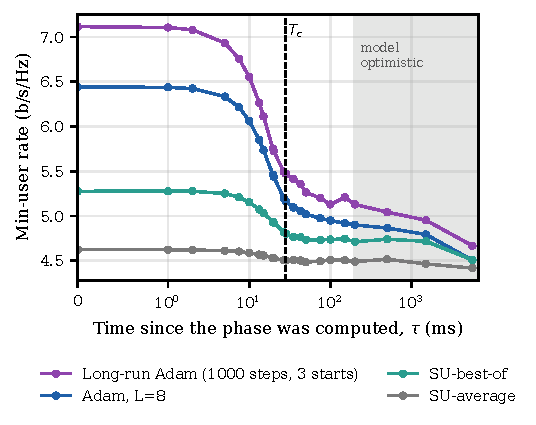
\includegraphics[width=0.92\columnwidth]{figures/fig_aging.pdf}
\caption{Minimum user rate of a phase fixed at $t=0$ as users walk at 1.5~m/s, with the precoder refreshed. Dashed: $T_c=28.2$~ms. Shaded: beyond 200~ms the model is optimistic.}
\label{fig:aging}
\end{figure}

\subsection{Optimal Number of Iterations}
\label{sec:res_optimum}
Fig.~\ref{fig:optimum} sweeps the number of Adam steps from SU-average (4.624~b/s/Hz). The $t=0$ rate rises with every step, from 5.412 at $L=1$ to 7.037~b/s/Hz at $L=48$. The effective rate does not: it peaks at $L=4$--$6$ (5.980, 5.982 and 5.970~b/s/Hz, at 6.7--10.0~ms), and every other step count is significantly lower. At $L=48$ it is 14.0\% (95\% CI 12.5--15.5\%) below the peak, although the $t=0$ rate there is 13.2\% higher. In terms of~\eqref{eq:marginal}, going from $L=4$ to $6$ adds 0.188~b/s/Hz at $t=0$ but costs 0.198 in aging.

The optimum is not an artifact of Adam or its step size. Step sizes 0.25, 0.75 and 1.0 put it at $L=6$, $4$ and $5$, with losses of 11.5\%, 13.7\% and 11.3\% at $L=48$. Armijo steepest ascent peaks at $L=4$ (6.015~b/s/Hz). It gains more than Adam in the first steps but costs 1.26 times as much per step, and the two peaks are statistically tied (difference 0.033, CI $-0.001$ to 0.064). With Armijo's per-step cost at 1.0, 1.2, 1.4, 1.6 and 2.0 times Adam's, its best effective rate is $+0.147$, $+0.050$, $-0.013$, $-0.079$ and $-0.197$~b/s/Hz relative to Adam's: even between two classical optimizers, latency decides the ranking.

\begin{figure}[t]
\centering
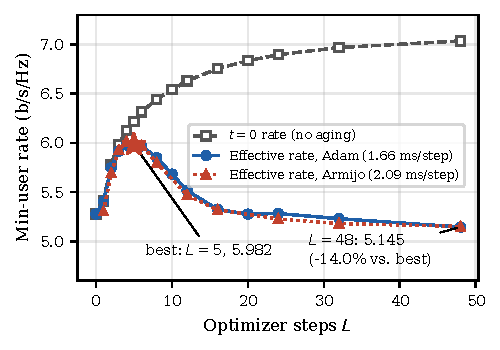
\includegraphics[width=0.92\columnwidth]{figures/fig_intrinsic_optimum.pdf}
\caption{Step sweep (aging set). The $t=0$ rate increases with $L$; the effective rate peaks at $L=4$--$6$ and is 14.0\% lower at $L=48$. Armijo (2.09~ms per step) shows the same shape. $L=0$: SU-best-of at 0.05~ms (5.276; 5.272 at its measured 2.5~ms).}
\label{fig:optimum}
\end{figure}

\subsection{Scaling of the Optimum with the Normalized Step Cost}
\label{sec:res_scaling}
An optimized implementation would be faster per step. Fig.~\ref{fig:scaling} therefore scales Adam's step time from 0.01 to 3 times the measured value, i.e., $x$ from $2.5\times10^{-4}$ to $7.5\times10^{-2}$; this setup sits at $x=2.5\times10^{-2}$, and the same axis covers users up to 100 times slower or 3 times faster than here. The best step count falls steadily: 96 steps at the smallest $x$, 48, 24--32, 12--16, 4--6 here, and 2 at the largest. At the smallest $x$ running to convergence costs little (running to $L=256$ costs 1.5\%, CI 1.3--1.8\%); the cost of convergence peaks at about 21\% near $x\approx 2.5\times10^{-3}$. For $x\ge 2.5\times10^{-2}$, $L=256$ lies beyond the 200~ms horizon, so its cost is, if anything, understated. Whether convergence hurts is therefore a property of the regime, not of RIS optimization in general. Faster hardware, such as a GPU or an NPU, shortens the step and so moves the optimum, but does not remove it: in the model (Proposition~1) an interior optimum exists for every $x>0$, and in the measurements it persists down to a hundredfold faster step, where it lies at 96 steps.

Both laws behind Proposition~1 hold approximately. The aging loss is close to quadratic ($R^2\ge 0.98$ for every $L$, fitted for $\tau\le 10$~ms), with $\kappa_L$ growing from 7.8 at $L=1$ to 25.1 at $L=48$. The convergence gap roughly follows a power law, with $\gamma=0.93$, but between 0.56 and 1.19 depending on the fit range, so the predicted exponent lies between $-0.78$ and $-0.63$. The measured slope of $L^\star(x)$ is $-0.675$ (95\% CI $-0.692$ to $-0.655$), inside that range; the model thus pins the exponent down only to about $\pm 0.08$. The closed form~\eqref{eq:Lstar} is within a factor of 1.27 of the measured optimum at every $x$ (5.3 against 5 here). This is an in-sample check: $\kappa_L$ is fitted over the delays (1.6--10~ms) at which the optima occur. The balance of Proposition~1 does not hold quantitatively (the ratio varies from 0.19 to 1.65), so the model explains where the optimum lies and why it moves, not how the two losses split.

A larger $8\times 8$ surface ($N=64$) raises the converged rate (8.48 against 7.10~b/s/Hz) but has the same best step count at every step-time multiplier, which confirms the optimum but not, independently, the exponent. Because its step costs only 1.04 times as much in our code, it sits at nearly the same $x$; an implementation whose cost grows with $N$ would move it to fewer steps.

\begin{figure}[t]
\centering
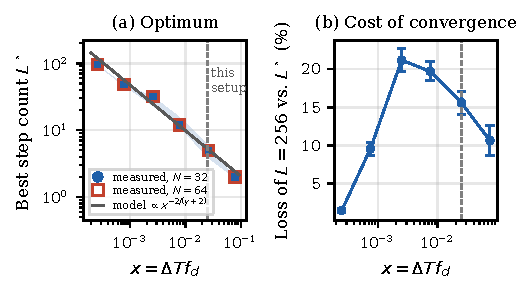
\includegraphics[width=\columnwidth]{figures/fig_step_scaling.pdf}
\caption{Adam with its step time scaled from 0.01 to 3 times the measured value. (a)~Best step count for $N=32$ (shaded: not significantly below the best) and $N=64$; line: closed form~\eqref{eq:Lstar}. (b)~Loss of running to $L=256$ instead of $L^\star$ ($N=32$), with 95\% paired CIs. Dashed: this setup.}
\label{fig:scaling}
\end{figure}

\subsection{Standardized Speeds and Acquisition Delay}
\label{sec:res_sensitivity}
Table~\ref{tab:speeds} repeats the main measurements on the same scenarios, on a time grid with 0.5~ms spacing up to 40~ms, at the speeds of the standards and two higher ones: 3~km/h, used in the 3GPP indoor-hotspot evaluation~\cite{3gpp_tr38913}; 10~km/h, the upper end of the IMT-2020 pedestrian class at which indoor mobility is evaluated~\cite{itu_m2410}; and, beyond the pedestrian class, 18~km/h (5~m/s, our choice in the vehicular class) and the 30~km/h of the dense-urban evaluation~\cite{3gpp_tr38913,itu_m2410}. Without acquisition delay, both findings---an optimal step count and the loss of the slow solvers---hold at every speed. The optimum moves from 8 steps at 3~km/h to 3 at 10~km/h, 2 at 18~km/h and 1 at 30~km/h. Running to $L=48$ costs 14.5\% (95\% CI 13.1--16.1\%) at 3~km/h and 10.5\% (9.0--11.9\%) at 10~km/h. SU-best-of is ahead of coordinate descent by 0.25--0.42~b/s/Hz and of long-run Adam by 0.45--0.69 at every speed, with paired CIs above zero (optimistic values for the slow solvers). At 18 and 30~km/h, $L=48$ lies beyond the reliable horizon (60 and 36~ms), so that cost is approximate. With 3.43~ms of acquisition delay the optimum is not resolved at 18 and 30~km/h, and at 30~km/h SU-best-of and coordinate descent are no longer significantly different. On this finer grid, $L=4$--$6$ are within 0.5\% of each other at 1.5~m/s, and running to $L=48$ costs 14.2\% (14.0\% in the main sweep).

\begin{table}[t]
\centering
\caption{Standardized and higher user speeds (aging set, no acquisition delay): coherence time, normalized step cost, best step count (range within 0.5\%), cost of running Adam to $L=48$, and $\Delta$: SU-best-of minus coordinate descent in effective rate (b/s/Hz). Computed on a 0.5~ms grid, so values can differ slightly from Table~\ref{tab:aging} and Fig.~\ref{fig:optimum}. $^\dagger$Beyond the reliable horizon; approximate.}
\label{tab:speeds}
\footnotesize
\setlength{\tabcolsep}{3pt}
\begin{tabular}{rlrrlrr}
\toprule
km/h & Source & $T_c$ (ms) & $x$ & $L^\star$ & $L{=}48$ & $\Delta$ \\
\midrule
3 & 3GPP~\cite{3gpp_tr38913} & 50.8 & 0.014 & 8 (6--8) & 14.5\% & $+0.27$ \\
5.4 & ours & 28.2 & 0.025 & 4 (4--6) & 14.2\% & $+0.31$ \\
10 & ITU~\cite{itu_m2410} & 15.2 & 0.046 & 3 & 10.5\% & $+0.25$ \\
18 & ours, ITU veh. & 8.5 & 0.083 & 2 & 8.0\%$^\dagger$ & $+0.42$ \\
30 & ITU, urban & 5.1 & 0.139 & 1 & 4.3\%$^\dagger$ & $+0.42$ \\
\bottomrule
\end{tabular}

\end{table}

A deployed system also spends time on pilots and feedback before it optimizes. On the main grid, adding an acquisition delay of 0--10~ms at 1--3~m/s moves the optimum the way~\eqref{eq:marginal} predicts (at 1.5~m/s from $L=4$--$6$ to $L=3$--$4$); excluding delays above $T_c/2$ (only 3~m/s with 10~ms), running to $L=48$ costs 2.9--14.7\%. The optimum also tolerates a wrong speed assumption: choosing $L$ for 1.5~m/s when users move at 1.8~m/s costs less than 0.5\%, and no pair of assumed and true speeds in our grid costs more than 5.7\%.

\emph{Shared scattering gains.} With one gain per scatterer for all BS antennas, as in a physical channel, absolute rates fall (Adam's best effective rate at 1.5~m/s on the grid of Table~\ref{tab:speeds}: 5.398 instead of 5.984~b/s/Hz), but the findings hold: $L^\star$ stays at 4--6 at 1.5~m/s and 3 at 10~km/h, running to $L=48$ costs 17.7\% (CI 15.8--19.5\%) and 14.2\%, respectively, and SU-best-of stays ahead of coordinate descent and long-run Adam (paired CIs above zero).

\subsection{Periodic Re-optimization}
\label{sec:res_tracking}
Table~\ref{tab:tracking} simulates the controller of Definition~3. The pilot overhead decides how often to update. With free pilots, back-to-back updates with two warm-started steps are best (6.36~b/s/Hz); with 0.86~ms of pilots the best period is 10--20~ms; with 3.43~ms, updates every 80~ms (warm start) and back-to-back updates with 48 steps (cold start) are statistically tied. What does not change is that short updates suffice: in every row some policy with at most 8 steps is not significantly below the best. Warm starting gains up to 0.53~b/s/Hz when pilots are short and nothing significant with 3.43~ms pilots.

\begin{table}[t]
\centering
\caption{Periodic re-optimization (aging set): best update period $U$ (ms; b2b = back-to-back) and steps per update $L$, with the time-averaged effective rate (b/s/Hz) for pilot durations $T_{\mathrm{p}}$. Warm$-$cold: paired difference of the two best policies; $^\S$not significant.}
\label{tab:tracking}
\footnotesize
\setlength{\tabcolsep}{5.5pt}
\begin{tabular}{r|rrr|rrr|r}
\toprule
 & \multicolumn{3}{c|}{Cold start} & \multicolumn{3}{c|}{Warm start} & \\
$T_{\mathrm{p}}$ (ms) & $U$ & $L$ & rate & $U$ & $L$ & rate & warm$-$cold \\
\midrule
0 & b2b & 3 & 5.83 & b2b & 2 & 6.36 & +0.53 \\
0.86 & 20 & 3 & 5.24 & 10 & 3 & 5.51 & +0.28 \\
1.71 & b2b & 48 & 5.08 & 20 & 3 & 5.17 & +0.09 \\
3.43 & b2b & 48 & 4.98 & 80 & 24 & 4.99 & +0.01$^\S$ \\
\bottomrule
\end{tabular}

\end{table}

\subsection{Learned Update Rule at Equal Steps and at Equal Latency}
\label{sec:res_reversal}
This comparison uses the static set and $t=0$ rates, to isolate compute efficiency. At an equal number of steps the learned rule outperforms tuned Adam at every budget $L\in\{1,2,4,8,16\}$ (Fig.~\ref{fig:eqms}(a)), winning on 68--84\% of test scenarios. But one learned step costs as much time as 2.7--4.0 Adam steps. On the measured time axis (Fig.~\ref{fig:eqms}(b)) every learned configuration is dominated by an Adam configuration that is both faster and better, in each of five timing rounds. For example, the learned rule with $L=4$ needs 18.41~ms for 5.285~b/s/Hz, while Adam with $L=8$ needs 13.48~ms for 5.380~b/s/Hz. The equal-step ranking reverses completely. Aging is not included here; since the learned configuration is the slower one in every pair, aging would be expected to widen the gap. The cost ratio, however, is a property of this implementation on one CPU thread: on hardware that accelerates the network's matrix products more than Adam's step, the reversal could weaken.

\begin{figure*}[t]
\centering
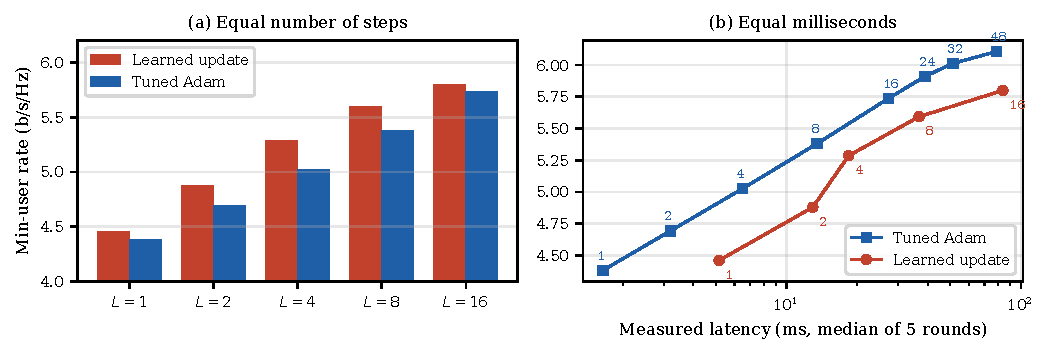
\includegraphics[width=\textwidth]{figures/fig_equal_step_vs_ms.pdf}
\caption{Learned update rule versus tuned Adam (static test set, 600 scenarios, $t=0$ rates, one CPU thread). (a)~At equal steps the learned rule is ahead at every budget. (b)~On the measured latency axis (labels: number of steps $L$), every learned configuration lies below and to the right of the Adam curve: it is dominated.}
\label{fig:eqms}
\end{figure*}

\subsection{Sensitivity to the Fresh-Precoder Assumption}
\label{sec:res_beam}
The main results assume that the BS refreshes its precoder from the current channel while only the RIS phase ages. On the beam set, keeping the precoder from $t=0$ instead makes the rate collapse within tens of milliseconds: at $T_c$ it is 11.7--14.2$\times$ lower than with a fresh beam, for every phase choice, and with the phase of Adam ($L=8$) a precoder only 5~ms old already lowers the rate from 5.228 to 1.736~b/s/Hz (beam-set rates are not comparable with Table~\ref{tab:aging}). Its computation is inexpensive (0.12~ms, about 13 times shorter than one Adam step), but it requires effective-channel pilots every few milliseconds; Section~\ref{sec:res_robust} charges their airtime.

\subsection{Robustness to Pilots, Estimation Error and Phase Resolution}
\label{sec:res_robust}
These checks use the aging set and the re-measured latencies of Section~\ref{sec:method} (1.33~ms per Adam step). Configurations are selected on an independent mobility draw (seed 12) and reported with paired CIs; $L^\star$ is read on the aging set.

\emph{Precoder pilots.} With the precoder refreshed every $T_{\mathrm{r}}$~ms from four pilot symbols that carry no data ($T_{\mathrm{r}}$ chosen per method) and the minimum user rate averaged over $W$~ms after deployment, net of pilots ($\bar{R}_W$), the selected configuration reaches 5.21~b/s/Hz with free refresh and 3.54, 4.00 and 4.33~b/s/Hz at 15, 30 and 60~kHz subcarrier spacing ($W=50$~ms, $T_{\mathrm{r}}=1$--2~ms). It uses 6--8 Adam steps; 3--20 steps are tied with it, and coordinate descent and long-run Adam are significantly behind. For $W=25$, 50 and 100~ms the selected step counts are 5, 6--8 and 16--20 (16--24 with free refresh); at 100~ms, with pilots, six steps lie 0.02--0.04~b/s/Hz below. Against SU-best-of, however, coordinate descent (deployed after 0.70~s, beyond the reliable horizon, where the model favors it) ties at $W=50$~ms with pilots and leads by 0.09--0.18~b/s/Hz with free refresh or at $W=100$~ms (except at 15~kHz); only tuned Adam beats coordinate descent under every window.

\emph{Imperfect channel knowledge.} With estimation error of power $1/(1+\rho)$ relative to the mean channel power ($\rho$: pilot signal-to-noise ratio; per-scenario median 22.6~dB for the RIS--user channel at 30~dB), the phase from the $t=0$ estimate and the precoder from a fresh one, the best effective rate falls from 6.08 to 3.54 and 1.40~b/s/Hz at 30 and 20~dB (the latter below the direct link alone, 1.74); at 10~dB and below rates are near zero and Adam and SU-best-of tie. With pilots charged as well ($\bar{R}_{50}$), Adam leads SU-best-of by 0.05--0.06~b/s/Hz at 30~dB and ties it at 20~dB; coordinate descent and long-run Adam stay significantly behind.

\emph{Discrete phases.} Rounding the phases of Adam (step size 0.5) and SU-best-of to $2^b$ levels at no time cost keeps an intrinsic optimum ($L^\star=5$, 6, 6 for $b=1$, 2, 3; $L=48$ costs 9.5, 14.1, 14.9\%). Discrete coordinate descent on the $2^b$ levels (16--501~ms) is significantly behind rounded SU-best-of at $b=3$, and at $b=2$ with two or more sweeps. At $b=1$ it is selected with a single sweep (16~ms): 0.25~b/s/Hz (CI 0.16--0.33) above rounded SU-best-of and tied with the best rounded Adam ($-0.04$, CI $-0.11$ to 0.02).

\section{Conclusion}
\label{sec:conclusion}

We asked which RIS phase optimizer a base station should run when users move, and for how long. Counting the time each method needs, we find the following.
\begin{enumerate}
    \item \textbf{Speed beats precision.} The solvers with the best rate on paper lose to a single-user heuristic that takes milliseconds, even with a tuned number of coordinate sweeps; without acquisition delay, this holds at every speed from 3 to 30~km/h (with optimistic values for the slow solvers). Averaged over longer windows, coordinate descent can tie or pass the heuristic but stays behind tuned Adam.
    \item \textbf{A few steps are optimal.} Adam's narrowband effective rate peaks after a handful of steps and then falls when the phase is renewed every few tens of milliseconds (holding it longer moves a flat optimum up); the optimum moves from 8 steps at 3~km/h to 3 at 10~km/h, the upper end of the IMT-2020 pedestrian class.
    \item \textbf{One number sets the optimum.} The best step count is governed by the step time relative to the Doppler frequency, $x=\Delta T f_d$, and scales approximately as $x^{-2/(\gamma+2)}$ (measured exponent $-0.675$); with a hundredfold faster implementation, convergence becomes nearly free.
    \item \textbf{Pilots set the update period.} In continuous operation the pilot overhead decides how often to update; each update should still be short.
    \item \textbf{Learning must win on the clock.} Winning at equal steps is not enough: the learned update rule (static set, one CPU thread) is dominated once each step is charged its measured time.
\end{enumerate}
In the regime quantified here, latency is not a secondary metric for mobile RIS: it decides which method is best.

\emph{Practical rules.} Choose the number of steps from $x$, the acquisition delay and how long the phase will be held, not from convergence. Choose the update period from the pilot overhead. Compare methods on measured latency against a classical baseline tuned at each budget, and report dominance rather than equal-step wins.

\emph{Limitations.} Fixed scatterers make long-horizon rates, and independent per-antenna gains absolute rates, optimistic; the findings hold with shared gains. The main results assume that the BS recomputes its precoder from the current channel with perfect knowledge. Pilot airtime (17--32\% lower rates), estimation error and 2--3-bit phases leave the slow solvers behind; at one bit a single-sweep search ties the best rounded Adam, and at pilot signal-to-noise ratios of 10~dB and below the fast methods cannot be told apart (Section~\ref{sec:res_robust}). RIS switching time is not modeled, and there is one geometry. Latencies come from single-threaded Python: compiled alone (62--63-fold faster), coordinate descent overtakes Python Adam, but an equal speed-up of all methods keeps tuned Adam ahead; the normalized step cost carries the results to other speeds and, approximately, carriers. Semidefinite relaxation~\cite{Wu2019TWC}, WMMSE~\cite{Choi2024TCOM} and manifold methods were not timed, and long-run Adam only at a fixed budget. In a first OFDM check the interior optimum held for centre-frequency optimization at 20~MHz, but at 50--100~MHz 48 steps were significantly worse in only 3 of 16 configurations.


\section*{Acknowledgment}
\emph{Use of AI tools.} In accordance with IEEE policy, we disclose that the AI assistant Claude (Anthropic) was used in preparing this article: to draft and edit the text of all sections, to port the authors' simulation framework to Python, to develop the experiment and analysis scripts in collaboration with the authors, who specified the experiments and checked the results, to generate figures and tables from stored results, and to check references. The authors designed the study, directed all analyses, verified every result and reference, and take full responsibility for the content.

\section*{Data and Code Availability}
The scripts that generate every table and figure, and the stored measurement files they read, are available at \url{https://github.com/sedasavascisen/ris-latency-mobility}.

\bibliographystyle{IEEEtran}
\bibliography{references/references}

\end{document}
